\chapter{Introduction}
\label{chap:Introduction}
%\section{Motivation}   
%\label{sec:Motivation}
The mesolimbic dopamine pathway comprising the ventral tegmental area (VTA) and its projections terminal to the ventral striatum (VS) has been identified as a critical neural system involved in processing both the behavioral effects of rewarded and unrewarded stimuli (\cite{Schultz1992}, \cite{Montague}, \cite{Ungless2004}, \cite{Sun2014}, \cite{Tobler2003}, \cite{UchidaDop1}, \cite{Takahashi2016}). The brain performs here a simple arithmetic: it compares the expected and the received outcomes and computes the differences between the two. In other words after receiving the outcome, it computes the error made in predicting the outcome. This computation is called reward prediction  error (RPE): it is essential to learning, to reward maximization, and to guide reward-related behavior. RPE has been widely investigated in last decades (\cite{Schultz1997}, \cite{UchidaDop}, \cite{Fiorillo}, \cite{Pagnoni}, \cite{Schultz2016}). In dopamine neurons RPE signals are characterized by activations following primary rewards and sensory reward-predicting stimuli. Dopamine neurons fire phasic burst within 100-500 ms after unpredicted rewards or cues that predict reward. Fiorillo and collaborators used distinct stimuli indicating the probability of reward, to show that the phasic activation of dopamine neurons varied monotonically across the full range of probabilities(\cite{Fiorillo}). Figure \ref{fig:probDopamine} (left) displays a dopamine neuron$'$s responses to stimuli with different reward probabilities. This response to reward is reduced when a reward is fully predicted (\cite{Uchida}). The prediction signal at stimulus onset increases when uncertainty about outcome decreases.\\These observations have defined the basis of the current knowledge on dopamine neurons, which are assumed to signal discrepancies between expected and actual rewards, in other words they are thought to compute the RPE.\\The prediction-related activation is usually preceded by a brief detection component before the proper valuation of stimulus: the RPE signal evolves in time from unselective sensory detection to more demanding and crucial stages of identification and valuation (\cite{Tobler2003}, \cite{Nomoto2010}, \cite{Fiorillo2013}, \cite{deLafuente}, \cite{Schultz2016}). This value is constantly adapted during the learning process by dopamine neurons (\cite{Tobler2005}). The initial component, characterized by a brief activation, occurs unselectively in response to a large variety of unpredicted events and corresponds to the large range and heterogeneous nature of potentially rewarding stimuli and object present in the environment. This component reflects the detection of stimulus, regardless its relation with the reward.
\begin{figure}[H]
    \centering
    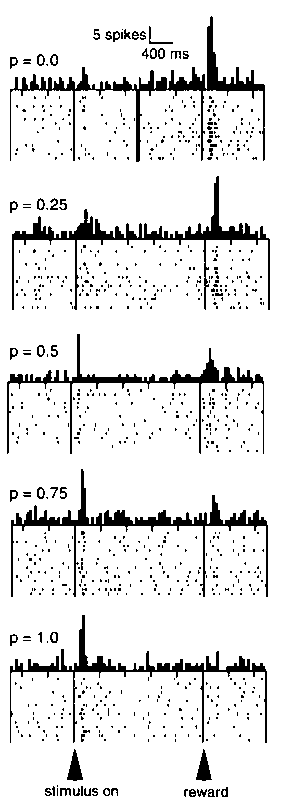
\includegraphics[scale=0.55]{figures/Schultz1.png}
    \hspace{1.5cm}
    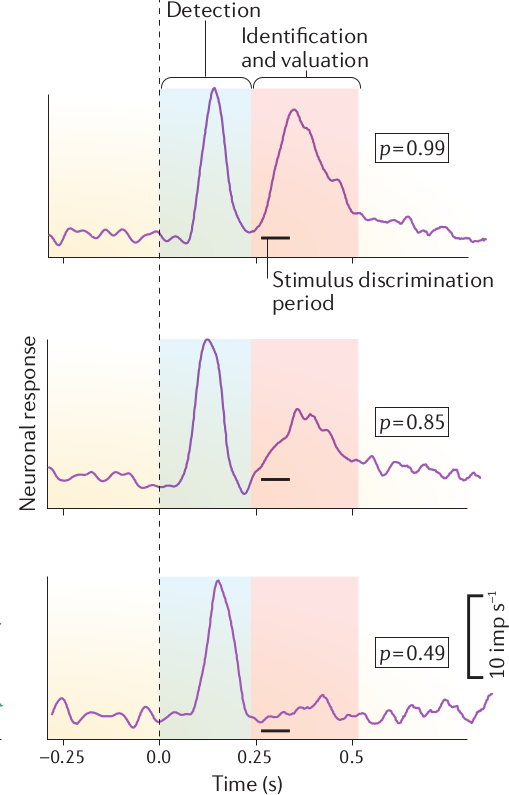
\includegraphics[scale=0.35]{figures/ResponseProbSchultz.png}
    \caption{\textbf{Left:} Adapted from \citeay{Fiorillo}: Reward-related responses of dopamine neurons. Distinct stimuli were used to indicate the probability of reward (p increasing from top to bottom). Dopamine neurons signals varied monotonically across the full range of probabilities. At the stimulus onset, the dopamine response increased monotonically as the probability increased; at the reward time instead, the dopamine response decreased monotonically as the probability increased. \textbf{Right:} Adapted from \citeay{Schultz2016} and \citeay{deLafuente}: A demanding random dot motion discrimination task reveals completely separated dopamine response components. Larger responses correspond to higher reward probabilities (p). The initial, stereotyped, non-differential activation reflects stimulus detection and decreases back to baseline (blue zone); the subsequent separate, graded increase develops when the animal signals stimulus discrimination; it codes reward value (red zone), which in this case derives from reward probability}
    \label{fig:probDopamine}
\end{figure}
The second component, also called main component or valuation component, defines the function of the dopamine response and reflects the evolving neuronal processing that is required to appreciate the value of the stimulus. Thus, at this stage the stimulus is identified and valued. Figure \ref{fig:probDopamine} (right) shows the separation between the detection and the valuation component of RPE signals in dopamine neurons.\\\\Like VTA neurons, neurons in ventral striatum show as well reward-related responses. In monkey experiments first it has been shown that VS neurons predominantly fire in relation to the expectation of reward (\cite{Schultz1992}). This signals suggested that VS neurons evaluate reward and reward-associated stimuli, and thereby participate in the processing of information underlying the RPE computation.\\The stereotypical responses of striatal projection neurons in VS during learning consist of a sustained increase of activity following stimulus onset before the occurrence of the reward delivery (see figure \ref{fig:StriatumN}).
\begin{figure}[H]
    \centering
    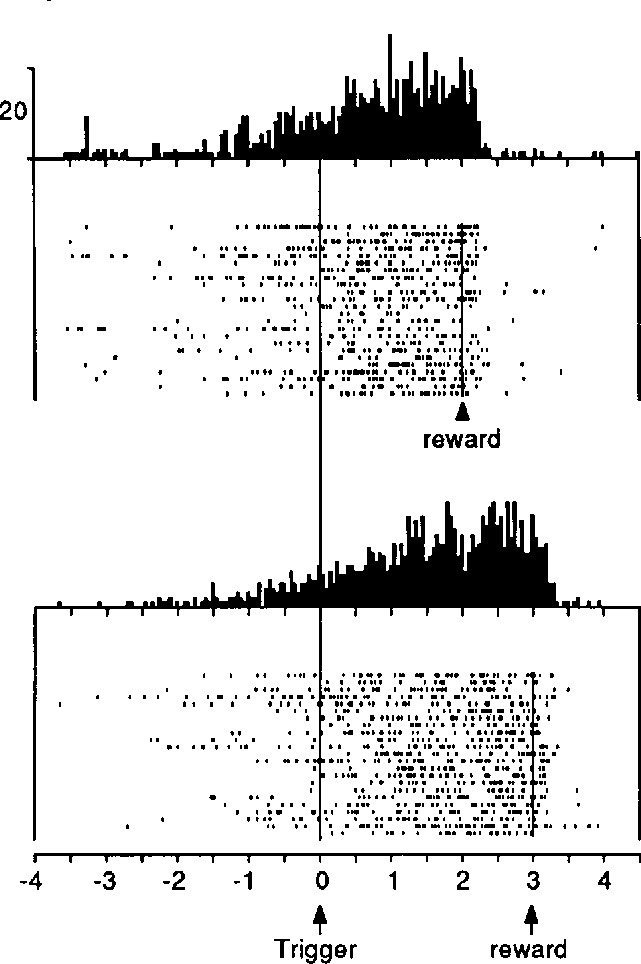
\includegraphics[scale=0.22]{figures/StriatumR.png}
    \caption{Adapted from \citeay{Schultz1992}. Stereotypical reward-related VS neuronal activity. Effect of delayed reward delivery in go/no-go task in monkeys. VS neurons show sustained increases of activity before the occurrence of individual task events. VS neurons exhibit activation in relation to the expectation of reward.}
    \label{fig:StriatumN}
\end{figure}
The ventral pallidum (VP), contains neurons with fast spiking activity. VP it is innervated by dopamine inputs from the midbrain; and dopamine directly alters VP neuronal firing (\cite{Napier89}). In 1991, VP was assumed to integrate reward-related signals carried by VTA dopamine neurons, involved in reward-motivated behavior (\cite{Napier91}). This concept was quickly expanded to encompass the idea that dopamine transmission within the VP regulates a collection of behaviors, including locomotion and cognition (\cite{Napier92}). Contrary to the well-characterized, relatively homogeneous striatal projection neurons, the cellular architecture of VP is only beginning to be understood with its heterogeneous cell-types, neurotransmitters, and connectivity (\cite{Heimer1997}, \cite{Tachibana2012}). 
\subsubsection{Aim of the study}
While there is an extensive data on how RPE signals are expressed by single units, it remains elusive how the RPE computations are implemented in VS-VTA neural circuits (\cite{Schultz2016}). Thus, a better understanding VS-VTA related circuit activity will broaden our understanding on the underpinnings of RPE signals.\\\\In this work I studied the formation of prediction error signals in interregional assemblies during reinforcement learning. Towards this aim, I used dual site electrophysiological in-vivo data from VS (including ventral pallidum) and VTA, during a reversal go/no-go task in mice (unpublished data recorded by Max Scheller and Wolfgang Kelsch). Units in VS were classified as striatal projection neurons (SPN), fast spiking neurons (FSN) and cholinergic interneurons. Units in VTA were classified as dopamine neurons (DAN), gabaergic neurons (GABA) and glutametergic neurons.\\On this data set, I applied a cell assembly detection algorithm (\cite{RussoDurstewitz}). This statistical approach was built to detect spike patterns at any time scale and coordination, enabling the investigation of the time scales and the inter-units lag activation involved in the detected patterns of spikes. I focused the analysis on interregional assembly-pairs, namely assemblies formed by two neurons, one in VS and the other one in VTA. In this way I was able to examine the directionality between VS-VTA interactions through the inter-unit lag activation.\\\\I addressed the following questions in the thesis:\\\\Are specific cell-types more likely to aggregate into cell assemblies? And, if specific cell-types form distinct assemblies, do the assemblies in this specific composition occur more often than in other possible compositions?\\\\Do specific cell-types of one region lead the activation of other cell-types in another region? Towards this aim I studied the inter-unit lag activation distributions of each assembly-pair types. I used the time scale distribution of assembly-pairs to focus the analysis on the time scale in which the RPE signals are supposed to be encoded.\\\\Do assembly-pair types show specific task-related activity patterns that could reflect specific coding future? To this purpose, I examined the activity patterns of each assembly-pair type in relevant task moments.\\\\Finally to examine the learning dynamic of the task in the neuronal data, I employed a reinforcement learning model. Crucial terms of reinforcement learning are the uncertainty of the animal about the outcome and the reward prediction error. Both terms were modeled as time evolving components, in such a way that I could take into account the fact that during the task, the animal had to assign and re-assign new value to the presented stimulus. The proposed model was compared with other three models using the likelihood-ratio test (LRT), in the cases in which the models were nested, and the Bayesian information criterion (BIC) in cases the models had the same numbers of parameters.\\\\
Using regression of the assembly activity on the modeled uncertainty and the modeled prediction error, I asked whether different VS-VTA assembly types coded for RPE signals.

%I found that, in interregional assembly-pairs, VS predominantly led VTA. Moreover interregional assembly-pairs showed a bimodal time scale distribution, such bimodality was solely present in VS-VTA pairs and did not emerge in intraregional pairs.\\I examined the assembly-pair activity patterns of pairs with different time scales and directionalities. It emerged that different time scales and directionalities segregated different activity patterns. Specifically, in more precise time scale, directional assembly-pairs with VTA following VS showed excitatory responses following reward-predicting stimuli, in agreement with prediction error encoding.\\Taking advantage of neuron types classifications both in VS and VTA, I further investigated the specific cell-type composition of the assemblies exhibiting directionality. Interestingly only assembly-pairs formed by putative striatal projection neurons (pSPN) and dopamine neurons (pDAN) were directional in the direction of VS leading VTA.\\Thus, I looked at the task related activity patterns of different assembly-pair types; and I expected that, being directional, SPN-DAN assembly-pairs could exhibit RPE response.\\Indeed, different assembly-pairs types showed different activity patterns in response to external potentially rewarded stimuli. The segregation reflected different encoding features in different assembly-pair types.\\In particular, SPN-DAN assembly-pairs were mainly activated by the rewarded stimulus, and only a small fraction ($\sim12\%$) was activated by both stimuli. The activation started few hundred milliseconds after the stimulus onset and remained high for few hundred milliseconds ([100,400] ms). SPN-DAN activity pattern suggested that those pairs conveyed the valuation component of RPE signals (\cite{Tobler2003}, \cite{Nomoto2010}, \cite{Schultz2016}). Conversely, FSN-DAN assembly-pairs responded indistinctly to both stimuli, either showing a brief and phasic activation at the stimulus onset or being inhibited by one or both stimuli; these signals suggested that FSN-DAN pairs were involved in motivational and/or hedonic signals. Hence, I put forth the hypothesis that the assembly-pairs specialize in different aspects of the learning-related coding.\\%\\Detailed discussion will be presented in\hyperref[sec:TaskResp]{~Section \ref*{sec:TaskResp}} and\hyperref[sec:FalseAlCorrRej]{~Section \ref*{sec:FalseAlCorrRej}}.\\
%So far the description barely considered the dynamic of the learning process. In fact, reward prediction coding signals in dopamine neurons varied according to the probability to get the reward, which was often related to the uncertainty (\cite{Schultz1992}). Dopamine neurons in VTA as well as neurons in VS modified their activity in function to the difference between received and expected outcomes (\cite{Fiorillo}). In similar ways, far from being static, the assembly-pair activity modified itself trial by trial, reflecting the dynamic of the learning.\\This dynamic could not be replicated by the study of activity patterns, for this reason I modeled a reinforcement learning model. Crucial terms of reinforcement learning are the uncertainty of the animal to get the reward and the reward prediction error; the first is high when the animal is unsure about the outcome, and decreases as the animal becomes expert; the latter term reflects the ability of the animal to predict the reward: as the animal learnt is supposed to be able to predict the future outcomes. Both the aforementioned terms were modeled as time evolving components, in such a way that I could take into account the fact that, during the task, the animal had to assign and re-assign new value to the presented stimulus.\\Based on broad knowledge, reward prediction error signals are thought to be anti-correlated with the uncertainty of the animal to get the reward and correlated with the prediction error term of the Rescorla-Wagner models.\\Thus, if SPN-DAN assembly-pairs specifically encoded prediction error signals, I expected their activity to anti-correlate with the modeled uncertainty ($\alpha$) and to correlate with the modeled prediction error ($\delta$).\\Imodeled two linear Poisson regressions and I regressed the assembly-pairs activity on $\alpha$ and $\delta$. Our SPN-DAN assembly-pairs indeed anti-correlated with the uncertainty and correlated with the prediction error term. Furthermore I noted that such correlations were not found in other assembly-pair types, from which I could conclude that SPN-DAN assembly-pairs specifically conveyed reward prediction signals.  